\documentclass[platz]{tudphygp}
\usepackage{tudphymd,mhchem,listliketab}
\usepackage[normalem]{ulem}

\versuch{Passiver Zweipol}{PZ}

\begin{document}
\maketitle

\section*{Aufgabenstellung} 
\emph{Bei den zu untersuchenden Zweipolen handelt es sich um Reihen- bzw. Parallelschaltungen aus jeweils
einem ohmschen Widerstand und einem Kondensator oder einer Spule. �berlegen Sie sich also vor Versuchsbeginn, 
welches Verhalten $Z(\omega)$ und $\varphi(\omega)$ Sie f�r welche Schaltung erwarten!}
\begin{enumerate}
 \item Entsprechend der Anleitung in Ihrer Vorbereitung bestimmen Sie die Ortskurve des Zweipols mit Hilfe 
 eines Zweikanal-Oszilloskops und zweier Wechselspannungsmessger�te.\\
 Dazu bauen Sie nachfolgende Schaltung auf.
 \begin{figure}[h]
  \centering
  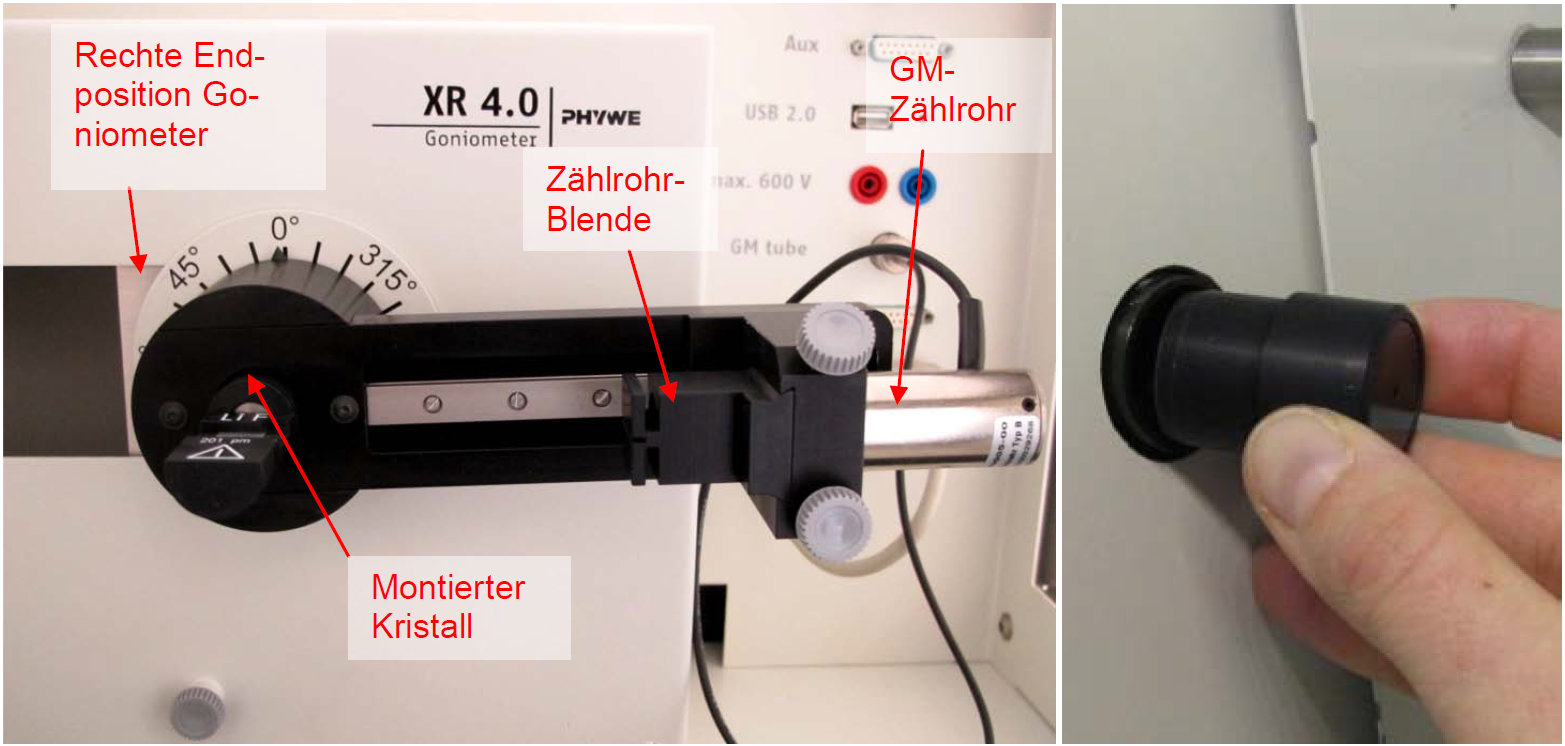
\includegraphics[width=0.7\textwidth]{aufbau.png}
 \end{figure}
 \item Nehmen Sie f�r einen am Platz liegenden Zweipol im Frequenzbereich $0<f<\SI{6000}{Hz}$ (10 bis 15 
 Messpunkte) die Spannungen $U_R(\omega)$ und $U_Z(\omega)$ und die Phasenverschiebung $\varphi(\omega)$ 
 (�berlegen Sie sich, wie man mit dieser Anordnung die Phasenverschiebung zwischen Strom und Spannung 
 �ber dem Zweipol messen kann) auf und berechnen Sie den Betrag $Z(\omega)$ des komplexen Widerstandes 
 $\uline Z(\omega)$.
 \item Stellen Sie anhand des Verhaltens $Z(\omega)$ und $\varphi(\omega)$ fest, ob es sich beim ausgemessenen
 Zweipol um eine
 \begin{itemize}
  \item Reihenschaltung oder Parallelschaltung aus Widerstand und Spule oder
  \item Reihenschaltung oder Parallelschaltung aus Widerstand und Kondensator handelt.
 \end{itemize}
 \item Zeichnen Sie die Ortskurve der Schaltung.
 \item Bestimmen Sie aus der Ortskurve die Werte und Fehlergrenzen des ohmschen Widerstan des und der 
 Kapazit�t bzw. der Induktivit�t in der Zweipolschaltung.
 \item Versuchen Sie die Ergebnisse evtl. durch eine sinnvolle Zusatzmessung zu verbessern.
\end{enumerate}

\section*{Fehlergrenzen der verwendeten Ger�te}
Der maximale Messfehler der Frequenz des Sinusgenarators ($\SI{200}{MHz}$ SINE-WAVE-GENERATOR, Hersteller HAMEG) 
ist durch die Anzeige dominiert und betr�gt $\pm\SI{1}{Digit}$.\\\\
Messgenauigkeit der Oszilloskope Tektronix TDS1000 und TDS2000
\begin{itemize}
 \item Zeitmessung:
 \begin{equation*}
  \Delta t=\num{0,004}\cdot t_E+\num{e-4}\cdot\left|t_A\right|+\SI{0,6}{ns}
 \end{equation*}
 \storestyleof{itemize}
 \begin{listliketab}
  \begin{tabular}{ll}
   $t_E\dots$ & Einstellwert der Zeitbasis, also z.B. bei ($\SI{5}{ms}$/Teilung) ist $t_E=\SI{5}{ms}$\\
   $t_A\dots$ & Ablesewert der Zeitmessung
  \end{tabular}
 \end{listliketab}
 \item Spannungsmessung:
 \begin{equation*}
  \Delta U=\num{0,01}\cdot U_E+\num{0,03}\cdot\left|U_A\right|+\SI{1}{mV}
 \end{equation*}
 \storestyleof{itemize}
 \begin{listliketab}
  \begin{tabular}{ll}
   $U_E\dots$ & Einstellwert des Spannungsmessbereichs, also z.B. bei ($\SI{5}{V}$/Teilung) ist $U_E=\SI{5}{V}$\\
   $U_A\dots$ & Ablesewert der Spannungsmessung
  \end{tabular}
 \end{listliketab}
 
\end{itemize}

\end{document}
